\documentclass[10pt, twocolumn]{article}

% ── Packages ─────────────────────────────────────────────────────────────────
\usepackage[T1]{fontenc}
\usepackage[utf8]{inputenc}
\usepackage{lmodern}
\usepackage[a4paper, top=1.8cm, bottom=2.0cm, left=1.5cm, right=1.5cm,
            columnsep=0.55cm]{geometry}
\usepackage{amsmath, amssymb}
\usepackage{graphicx}
\usepackage{booktabs}
\usepackage{array}
\usepackage{xcolor}
\usepackage{hyperref}
\usepackage{enumitem}
\usepackage{microtype}
\usepackage{caption}
\usepackage{float}
\usepackage{authblk}
\usepackage{titlesec}
\usepackage{fancyhdr}
\usepackage{abstract}
\usepackage{cite}

% ── Colours ───────────────────────────────────────────────────────────────────
\definecolor{aims-blue}{RGB}{0, 70, 127}

% ── Hyperref ──────────────────────────────────────────────────────────────────
\hypersetup{colorlinks=true, linkcolor=aims-blue,
            urlcolor=aims-blue, citecolor=aims-blue}

% ── Section spacing ───────────────────────────────────────────────────────────
\titleformat{\section}{\normalfont\large\bfseries\color{aims-blue}}
  {\thesection}{0.6em}{}
\titleformat{\subsection}{\normalfont\normalsize\bfseries}
  {\thesubsection}{0.5em}{}
\titlespacing*{\section}{0pt}{7pt}{3pt}
\titlespacing*{\subsection}{0pt}{5pt}{2pt}

% ── Header / footer ───────────────────────────────────────────────────────────
\pagestyle{fancy}
\fancyhf{}
\lhead{\small\color{gray} AIMS RIC — Doctoral Training School 2026}
\rhead{\small\color{gray} ML-ESS Technical Report}
\cfoot{\small\thepage}
\renewcommand{\headrulewidth}{0.4pt}

% ── Abstract ──────────────────────────────────────────────────────────────────
\renewcommand{\abstractnamefont}{\normalfont\bfseries}
\renewcommand{\abstracttextfont}{\normalfont\small}
\setlength{\absleftindent}{0pt}
\setlength{\absrightindent}{0pt}

% ── Captions ──────────────────────────────────────────────────────────────────
\captionsetup{font=small, labelfont=bf, skip=3pt}

% ── Lists ─────────────────────────────────────────────────────────────────────
\setlist[itemize]{noitemsep, topsep=1pt, leftmargin=*}
\setlist[enumerate]{noitemsep, topsep=1pt, leftmargin=*}

% ── Paragraph spacing ─────────────────────────────────────────────────────────
\setlength{\parskip}{3pt}
\setlength{\parindent}{0pt}

% =============================================================================
%  TITLE BLOCK
% =============================================================================
\title{%
  \vspace{-1.2em}%
  {\large\textbf{AIMS RIC — Doctoral Training School 2026}}\\[3pt]
  {\Large\bfseries\color{aims-blue} ML-ESS: A Multi-Agent AI Research Assistant}\\[3pt]
  {\normalsize Technical Report — April 2026}%
}

\author[1]{\textbf{Jérémie N. Landu}}
\author[1]{\textbf{Samuler Kargbo}}
\author[1]{\textbf{Cecilia Akyeampong}}
\author[1]{\textbf{Abigail Nunoo}}
\author[1]{\textbf{Lambert}}
\affil[1]{%
  \small African Institute for Mathematical Sciences —
  Research Innovation Centre (AIMS-RIC),
  Doctoral Training School 2026.
  \texttt{jeremy@aimsammi.org}
}
\date{}

% =============================================================================
\begin{document}
% =============================================================================

\maketitle
\thispagestyle{fancy}
\vspace{-0.8em}

% ─────────────────────────────────────────────────────────────────────────────
\begin{abstract}
ML-ESS is a full-stack AI system that automates end-to-end research: given a
natural language question, it orchestrates four specialised AI agents to search
the web, synthesise evidence, draft a structured report, and evaluate its
quality. Built as a \emph{working demonstration prototype} for the AIMS-RIC
Doctoral Training School 2026, the system exposes a REST API (FastAPI) and a
Next.js web interface supporting real-time progress tracking and multi-provider
LLM fallback. Every architectural decision prioritises clarity and modularity
over production hardening, leaving well-defined extension points for future
work.
\end{abstract}

\noindent\textbf{Keywords:} multi-agent systems, LLMs, automated research,
FastAPI, Next.js, retrieval-augmented generation.

\vspace{2pt}\hrule\vspace{4pt}

% =============================================================================
\section{Introduction}
% =============================================================================

Conducting research manually is time-consuming: it requires querying multiple
sources, extracting claims, resolving contradictions, and drafting a coherent
document. ML-ESS automates this workflow through a four-agent pipeline.
Related work — AutoGPT~\cite{autogpt}, CrewAI~\cite{crewai},
LangChain~\cite{langchain} — provides agent primitives but lacks a structured
evidence chain with quality scoring. Lewis \textit{et al.}~\cite{rag}
established RAG as the foundational pattern; ML-ESS extends it with typed
intermediate artefacts and a self-evaluating stage.

The prototype runs end-to-end on a laptop with a single API key. It is
designed as a \emph{teaching platform}: each component is inspectable, each
intermediate artefact is persisted, and adding a new research phase requires
only inserting a new agent function into the pipeline.

\textbf{Core objectives:}
\begin{itemize}
  \item Accept any research question in natural language.
  \item Autonomously gather and synthesise web evidence.
  \item Generate a structured Markdown report with citations.
  \item Score report quality on four dimensions (coverage, faithfulness,
    usefulness, hallucination rate).
  \item Deliver results via a clean web UI with real-time feedback.
\end{itemize}

% =============================================================================
\section{System Architecture}
% =============================================================================

The system comprises a Python/FastAPI backend and a Next.js frontend
(Figure~\ref{fig:arch}). The backend runs the four-agent pipeline in a
background thread, persisting state in SQLite (WAL mode). The frontend polls
the REST API every two seconds and renders the report when complete.

\begin{figure}[H]
  \centering
  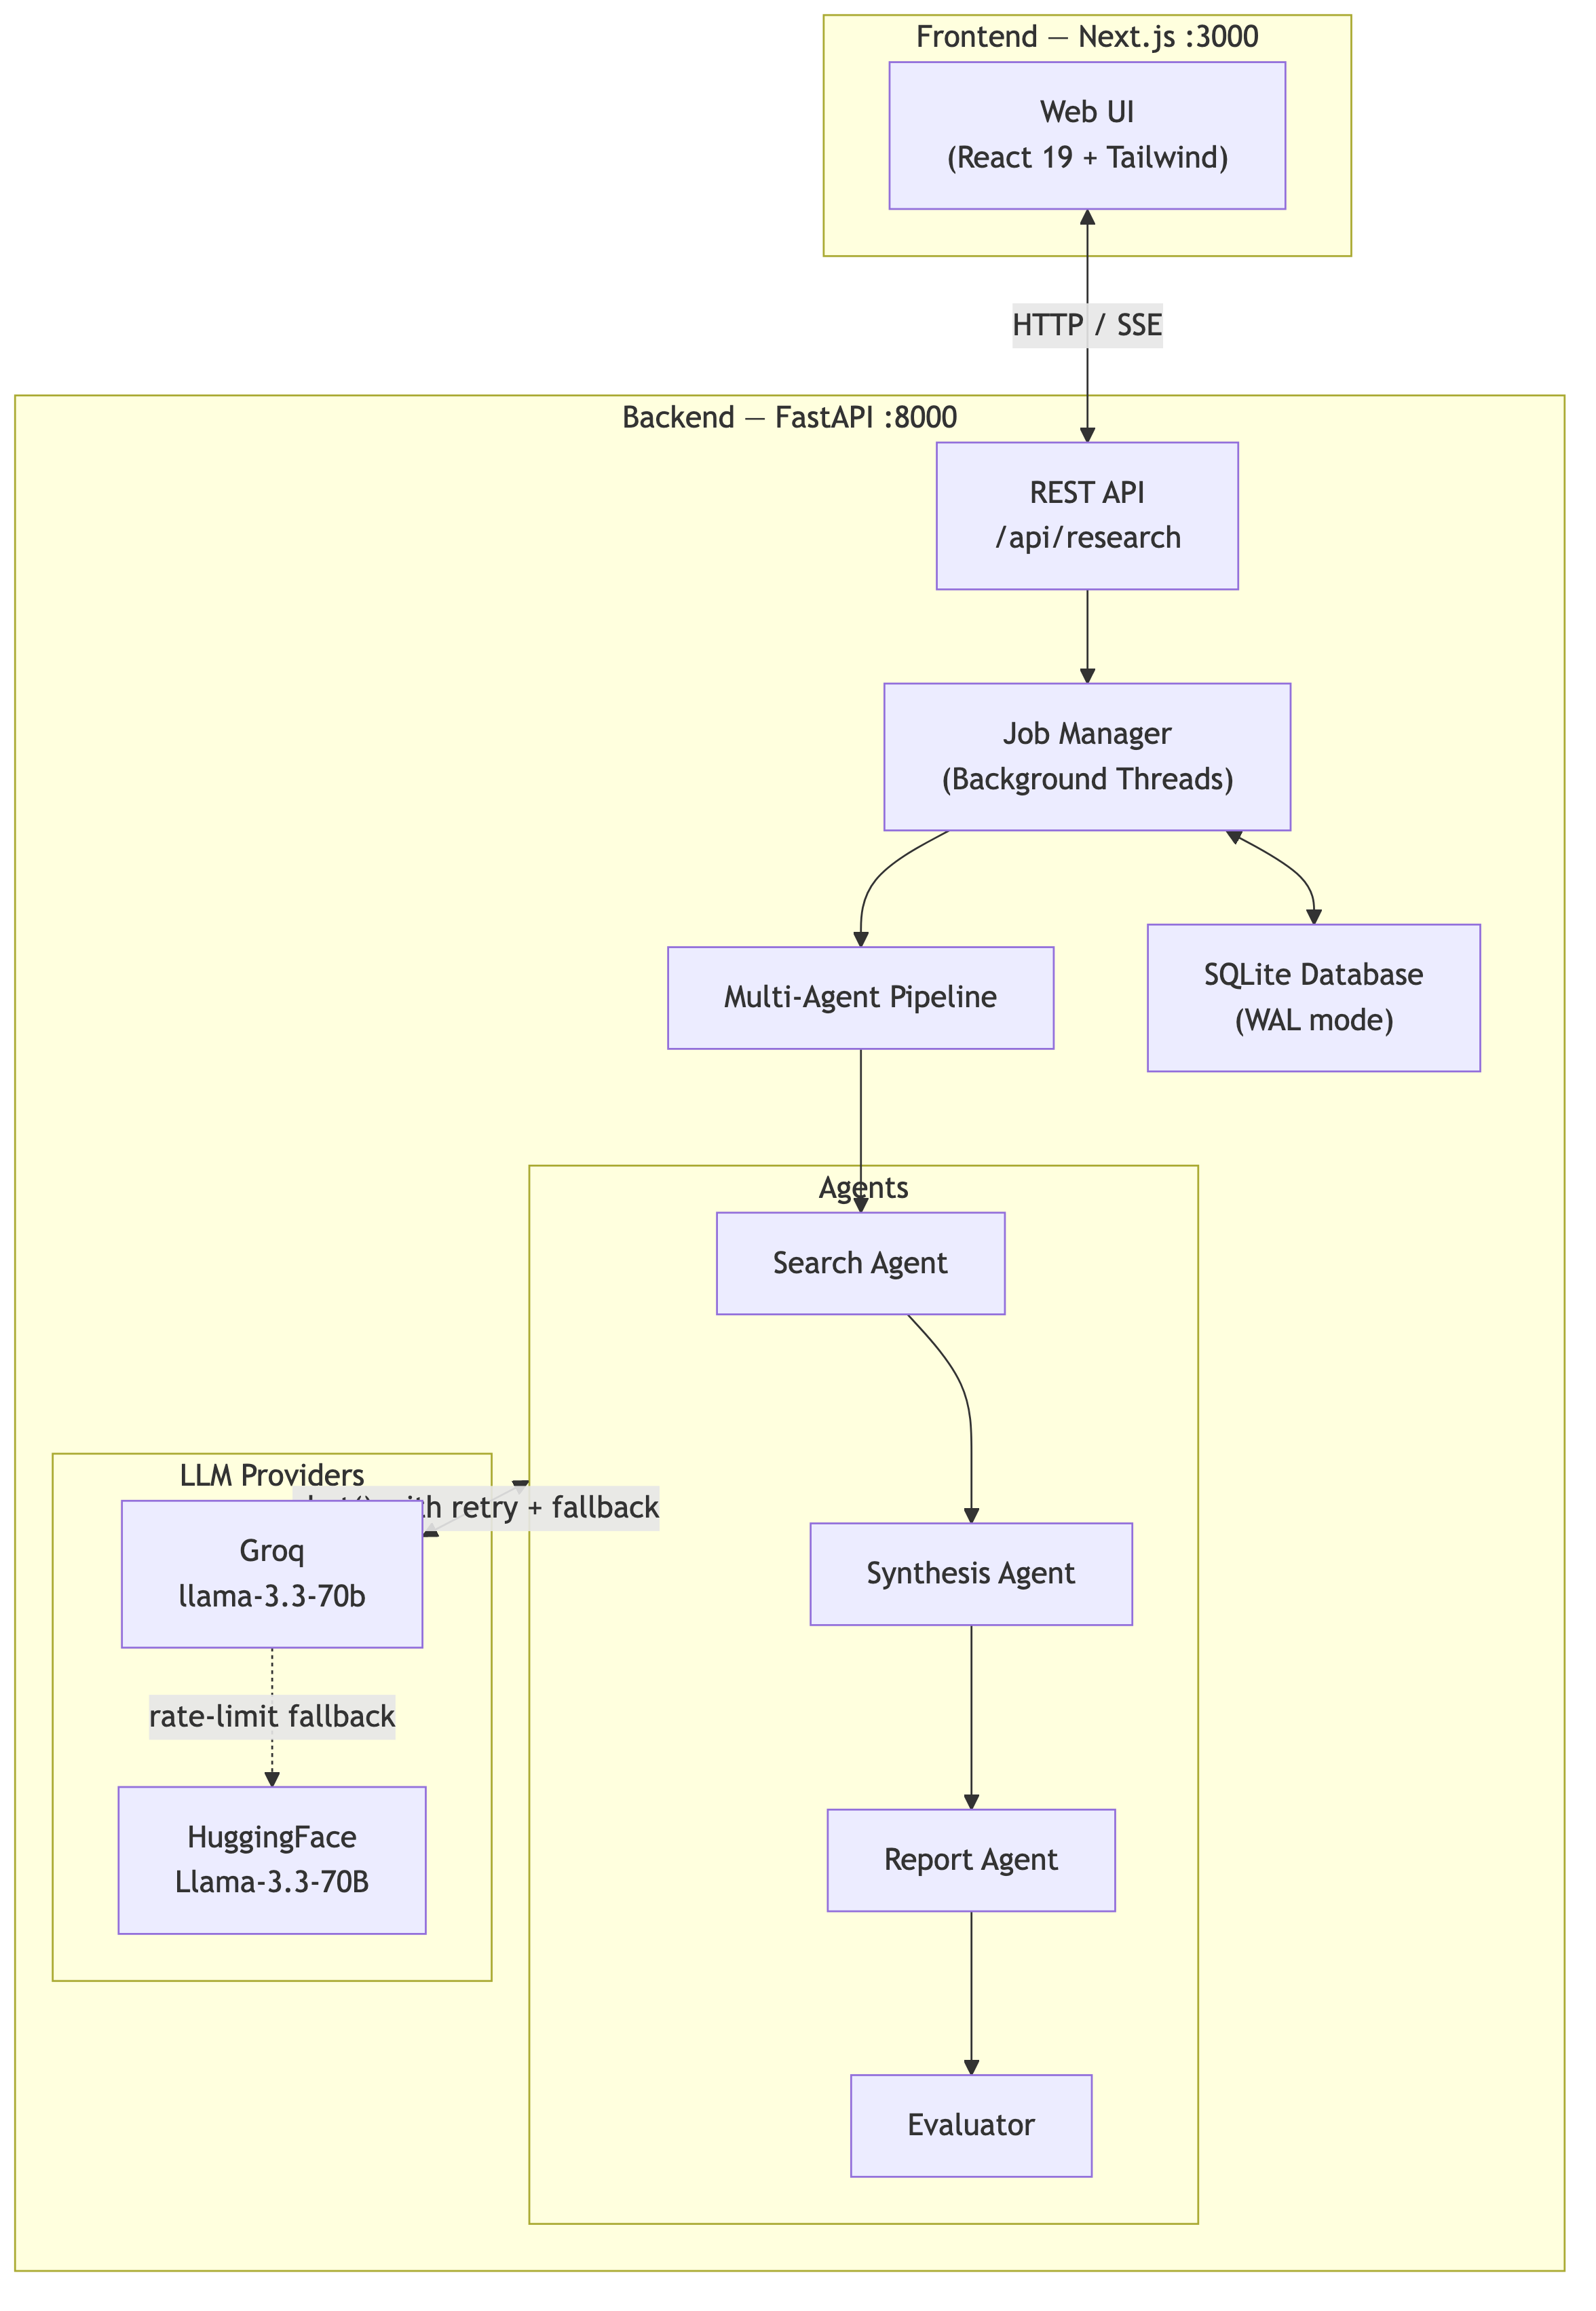
\includegraphics[width=\linewidth]{imgs/report-rendered-1.png}
  \caption{High-level system architecture.}
  \label{fig:arch}
\end{figure}

\textbf{Request lifecycle.} A \texttt{POST /api/research} request returns a
\texttt{job\_id} immediately (HTTP 202). A background thread runs the pipeline
and writes status updates to SQLite. The frontend polls
\texttt{GET /api/research/\{id\}} every 2\,s; an optional SSE stream at
\texttt{.../events} pushes stage-change events in real time.
Figure~\ref{fig:lifecycle} shows the full sequence.

\begin{figure}[H]
  \centering
  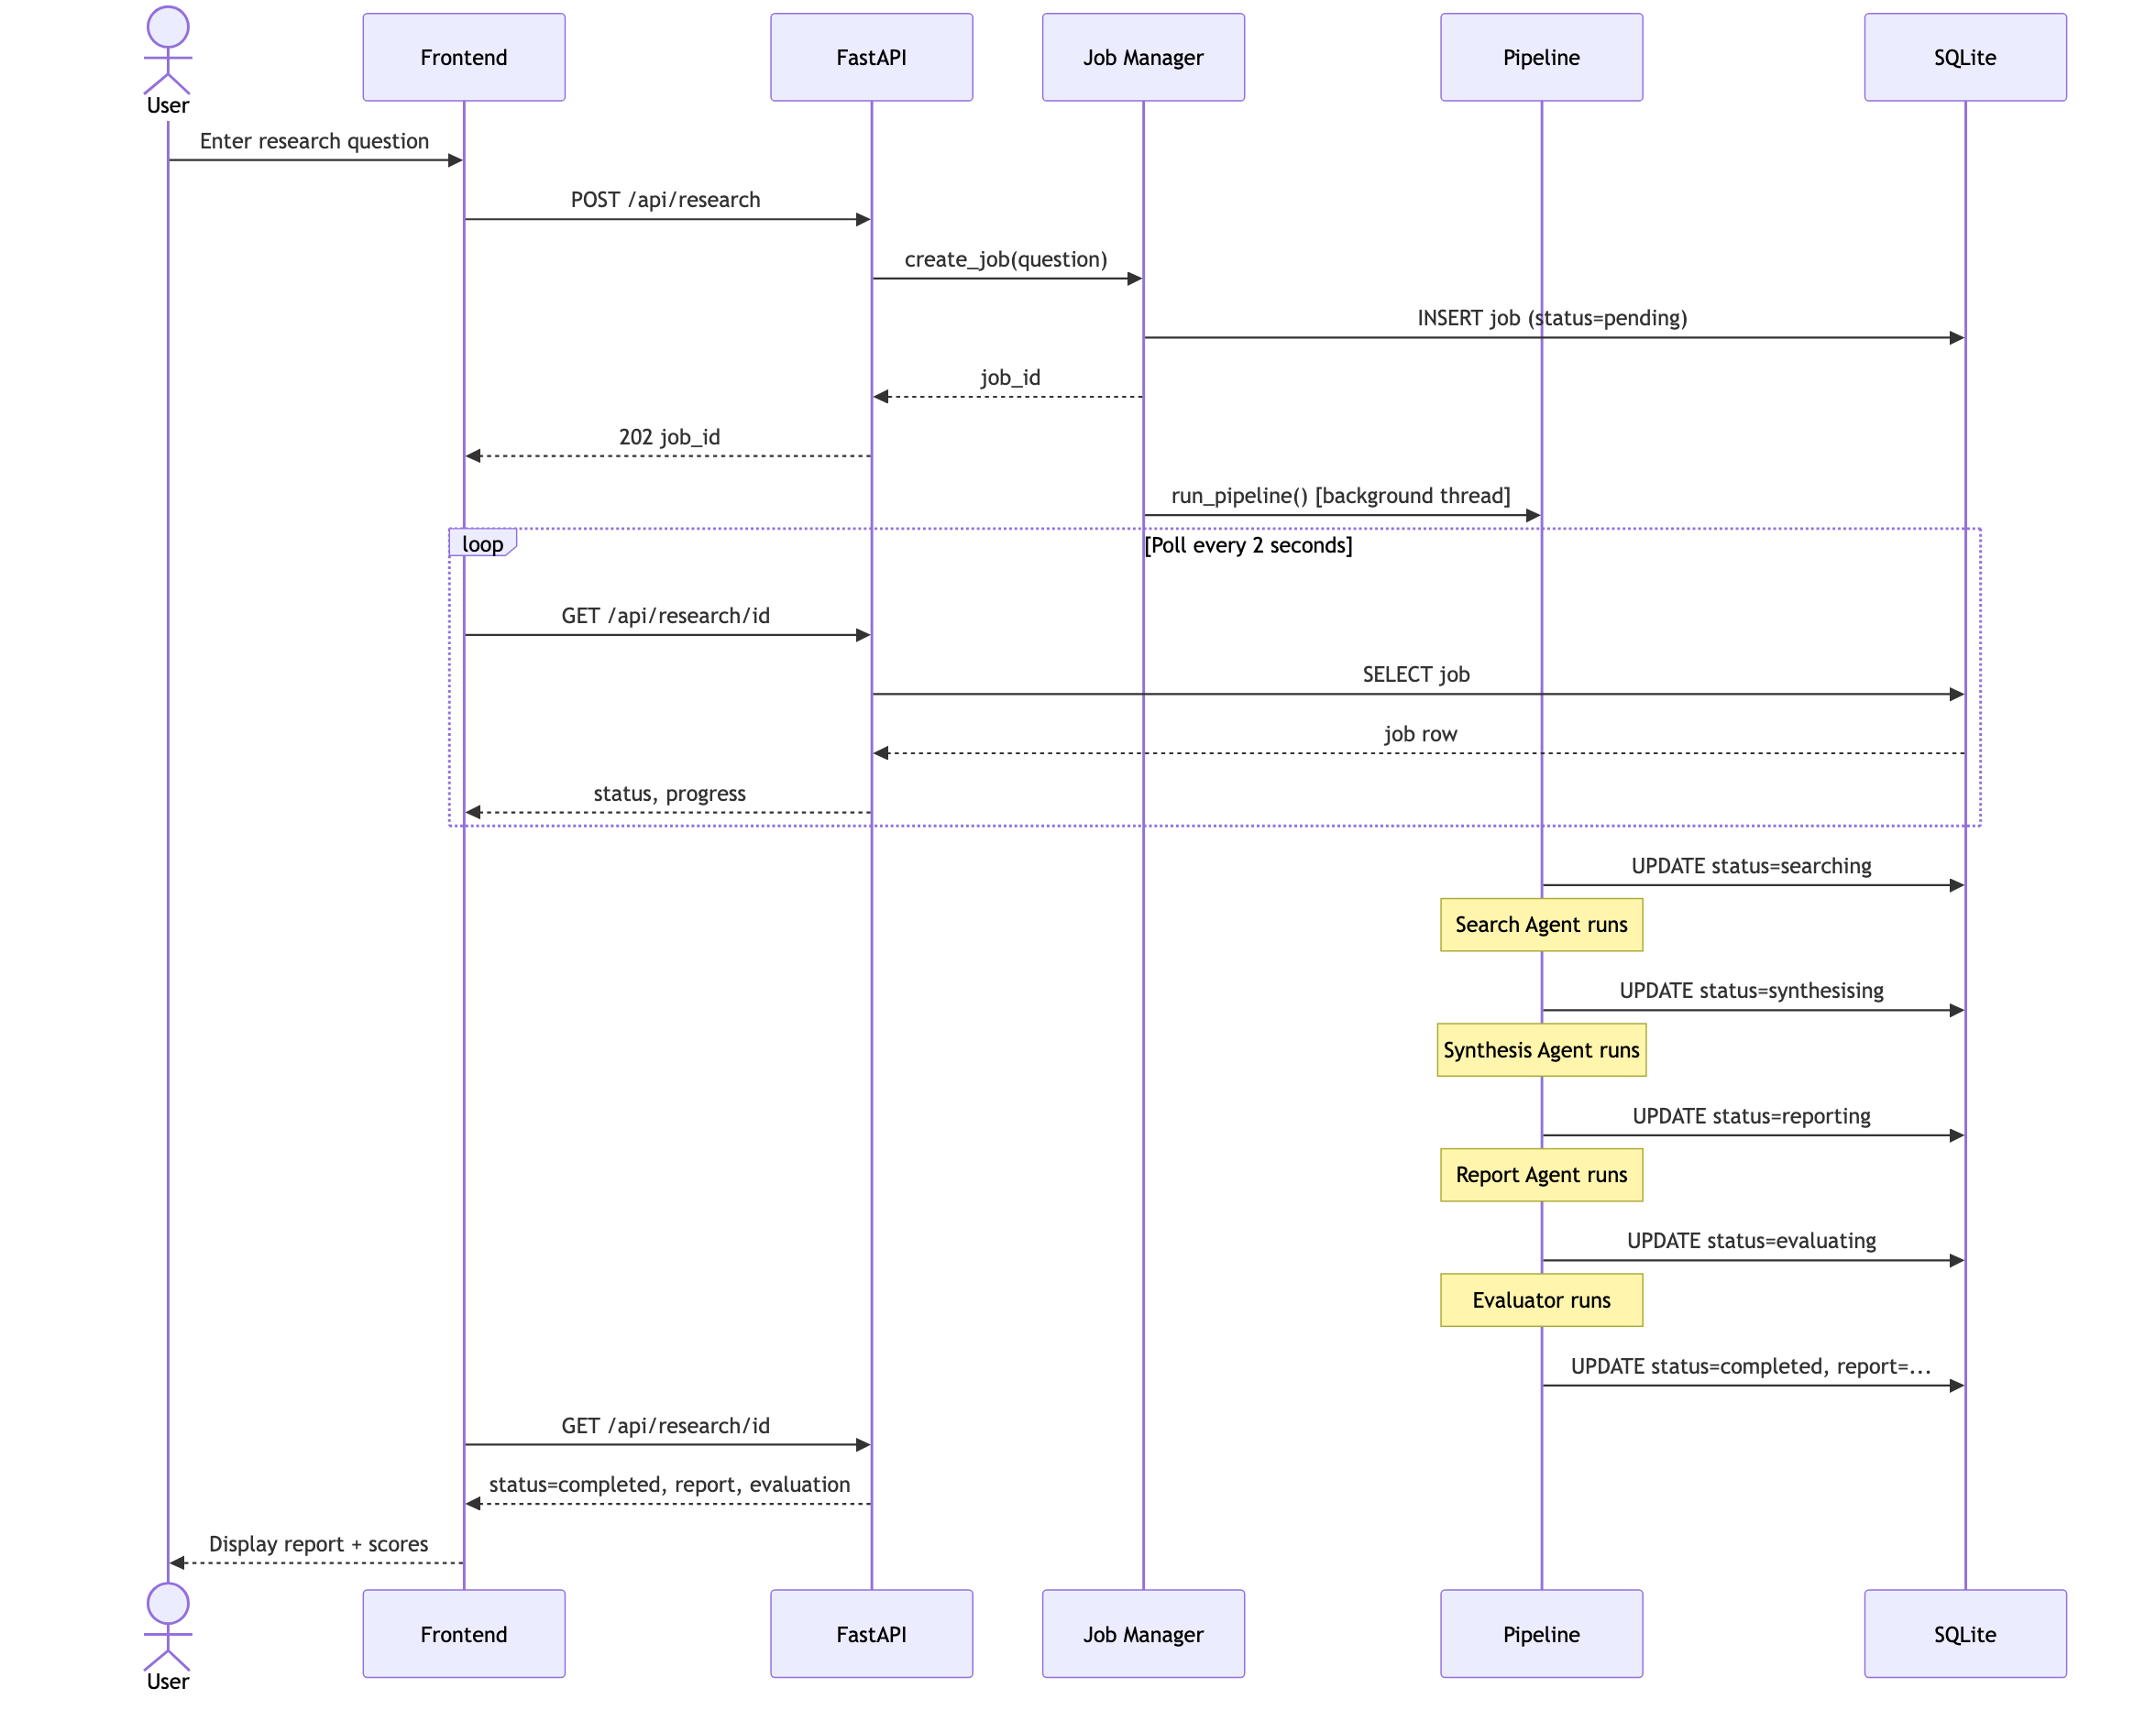
\includegraphics[width=\linewidth]{imgs/report-rendered-2.png}
  \caption{Request lifecycle sequence diagram.}
  \label{fig:lifecycle}
\end{figure}

\textbf{Backend layout} (\texttt{api/app/}): \texttt{agents/} — one file per
agent; \texttt{api/} — FastAPI factory, routes, SSE, auth;
\texttt{core/} — pipeline orchestrator, job manager, SQLite store, LLM client;
\texttt{models/} — Pydantic request/response and shared-state schemas.

% =============================================================================
\section{The Multi-Agent Pipeline}
% =============================================================================

\subsection{SharedState}

All agents share a single \texttt{SharedState} Pydantic object that travels
through the pipeline. It carries: \texttt{research\_question},
\texttt{search\_queries}, \texttt{sources} (title, URL, snippet, images,
credibility notes), \texttt{evidence} (claim, quote, relevance score,
source index), \texttt{themes} (name, summary, confidence: high/medium/low),
\texttt{contradictions} (description, resolution), \texttt{report\_outline},
\texttt{final\_report}, and \texttt{evaluation} (the four scores).
This typed contract makes each agent independently testable and the full
pipeline trivially extensible.

\subsection{Pipeline Flow}

Each agent is a stateless function that reads from and writes to the shared
\texttt{SharedState}. Figure~\ref{fig:pipeline} shows the four-stage flow.

\begin{figure}[H]
  \centering
  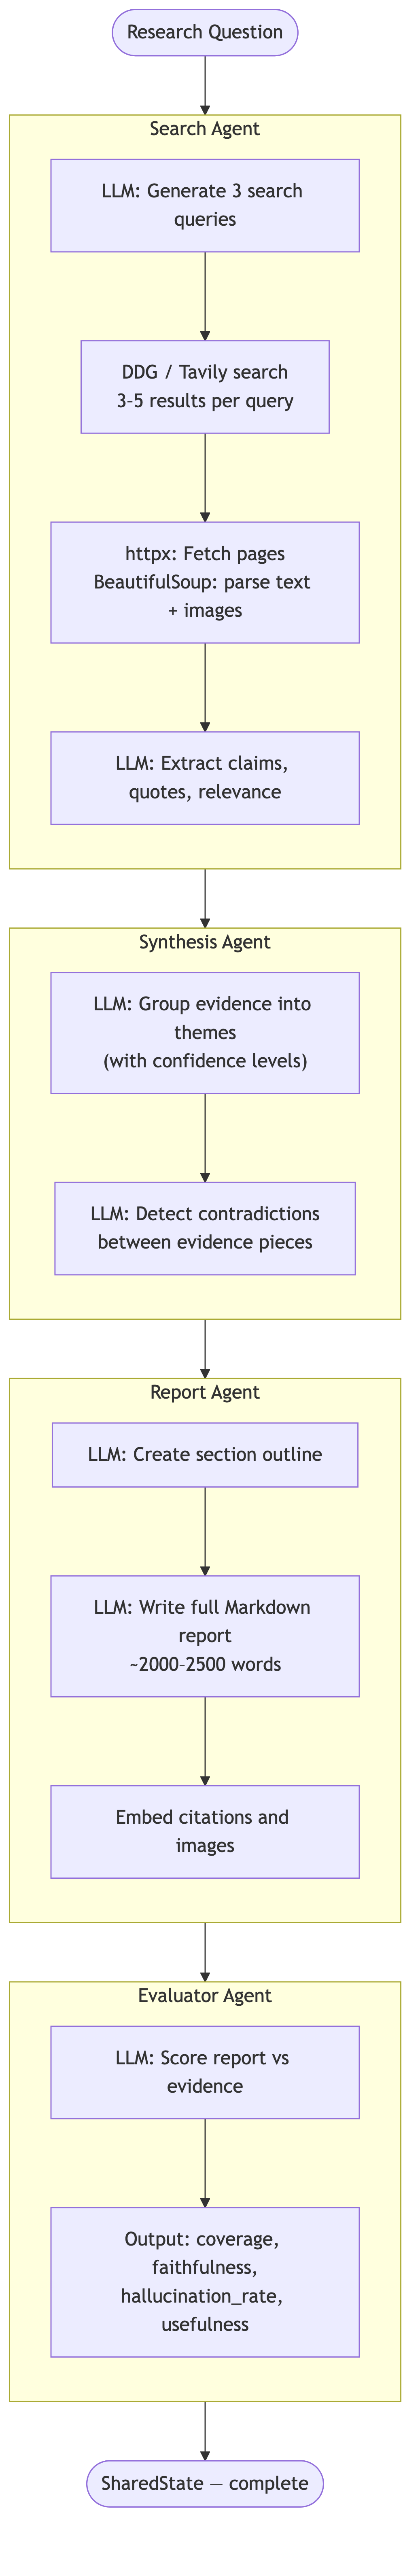
\includegraphics[width=0.5\linewidth]{imgs/report-rendered-4.png}
  \caption{Four-stage agent pipeline.}
  \label{fig:pipeline}
\end{figure}

\begin{enumerate}
  \item \textbf{Search Agent} — generates 3 queries via LLM, fetches up to 15
    pages (DuckDuckGo / Tavily), parses with BeautifulSoup4, extracts typed
    \texttt{Evidence} records.
  \item \textbf{Synthesis Agent} — clusters evidence into \texttt{Theme}
    objects with confidence levels; detects \texttt{Contradiction} pairs.
  \item \textbf{Report Agent} — builds a section outline then writes a
    \textasciitilde{}2\,000-word Markdown report with inline citations.
  \item \textbf{Evaluator} — scores the report against the evidence on
    coverage, faithfulness, hallucination rate, and usefulness.
\end{enumerate}

\subsection{Evaluation Scores}

The Evaluator outputs four scores in $[0,1]$ (Table~\ref{tab:scores});
lower is better for hallucination rate, higher is better for the rest.

\begin{table}[H]
  \centering\small
  \caption{Example evaluation output.}
  \label{tab:scores}
  \begin{tabular}{lc}
    \toprule
    \textbf{Dimension} & \textbf{Score} \\
    \midrule
    Coverage            & 0.87 \\
    Faithfulness        & 0.92 \\
    Usefulness          & 0.85 \\
    Hallucination rate  & 0.08 \\
    \bottomrule
  \end{tabular}
\end{table}

\subsection{Search Agent}

The Search Agent generates up to three LLM-crafted queries, fans them out to
DuckDuckGo (or Tavily when \texttt{TAVILY\_API\_KEY} is set), de-duplicates
up to 15 result URLs, fetches each page with \texttt{httpx} (10\,s timeout),
parses text and images with BeautifulSoup4, truncates to
\texttt{MAX\_CONTENT\_LENGTH} characters, and finally calls the LLM to extract
structured \texttt{Evidence} records (claim, quote, relevance score,
source index).

\subsection{LLM Provider Strategy}

Figure~\ref{fig:llm} shows the retry and fallback logic. Groq
(\texttt{llama-3.3-70b-versatile}) is the primary provider; HuggingFace
Inference serves as fallback when Groq's rate limit is exhausted.
Temperature is fixed at 0.3 for deterministic, reproducible outputs.
A secondary Groq key (\texttt{GROQ\_API\_KEY\_2}) can also be configured
to extend rate-limit headroom before falling back to HuggingFace.

\begin{figure}[H]
  \centering
  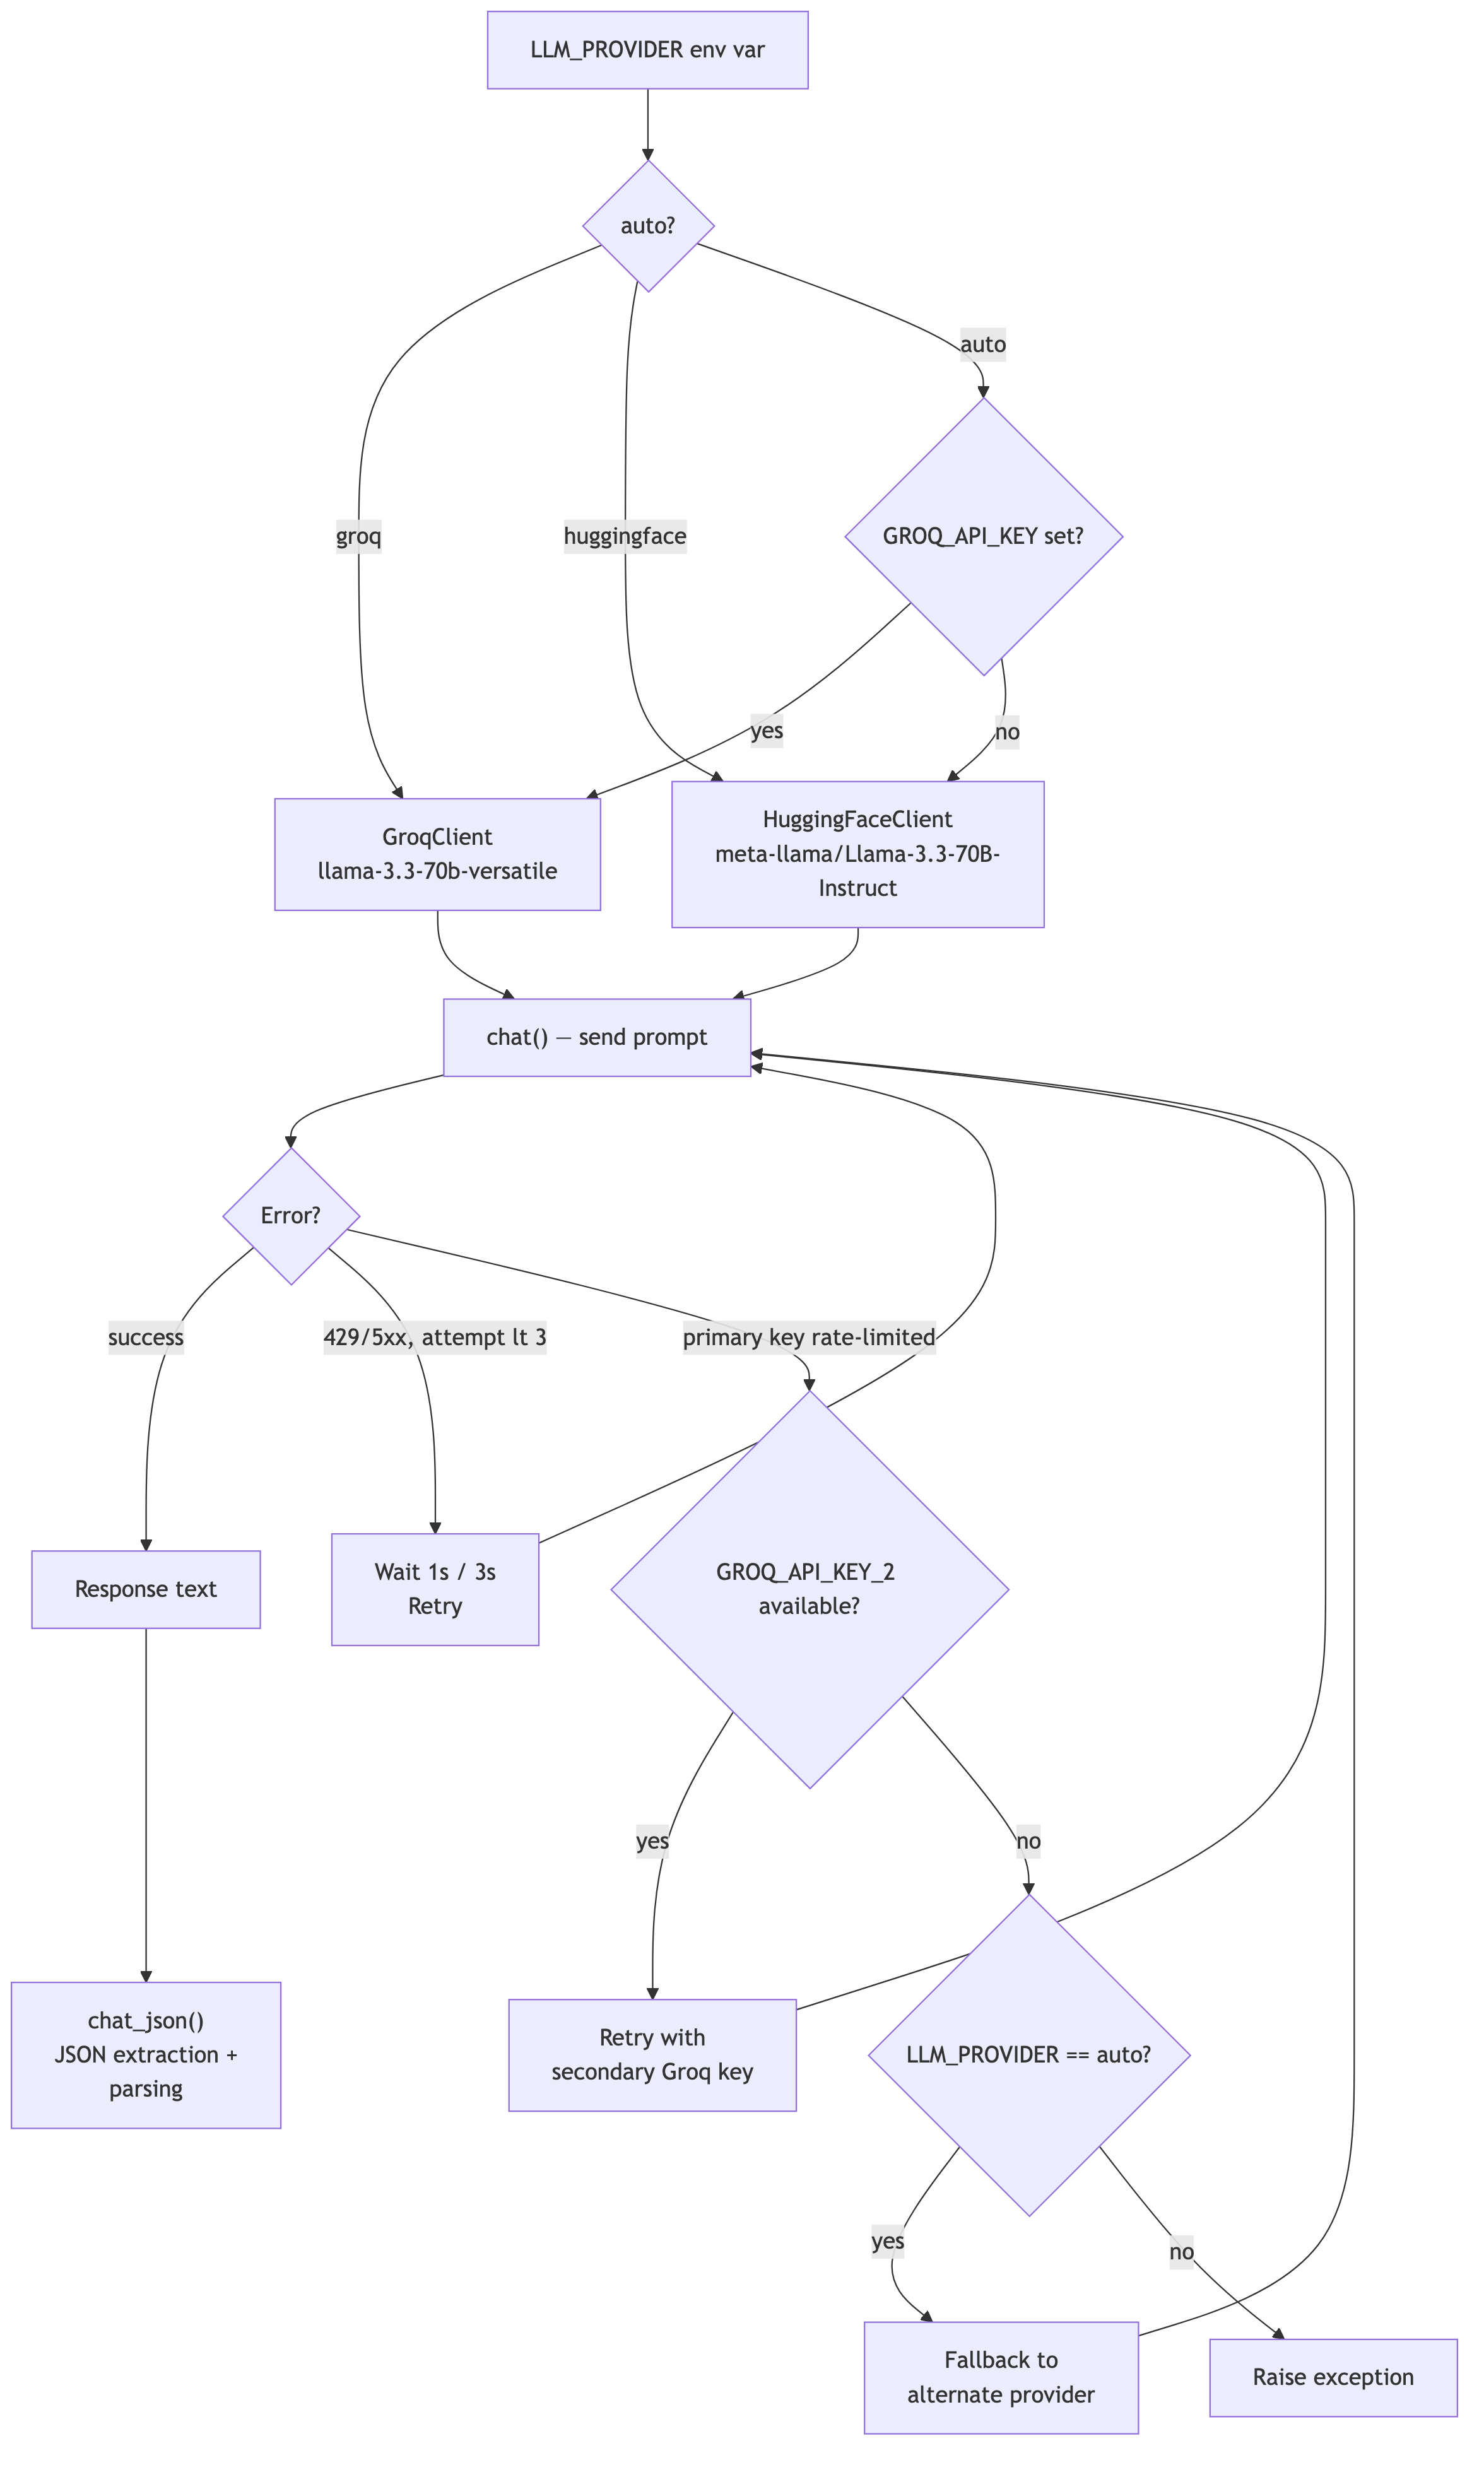
\includegraphics[width=\linewidth]{imgs/report-rendered-6.png}
  \caption{LLM retry and fallback strategy.}
  \label{fig:llm}
\end{figure}

% =============================================================================
\section{Data Persistence \& API}
% =============================================================================

\subsection{Schema}

The SQLite database has three tables. \texttt{JOBS} stores the primary record
(job ID, question, status, serialised report, evaluation scores, source/evidence/
theme counts, timestamps, error). \texttt{STATES} holds the full serialised
\texttt{SharedState} JSON for each job, enabling complete replay of any
pipeline run. \texttt{EVENTS} is an append-only log of SSE events emitted
during the pipeline (stage changes, queries ready, sources ready, job completed),
enabling the frontend to reconstruct the live event stream on reconnect.

\subsection{Job Lifecycle}

All job state is persisted in SQLite across the three tables above.
Figure~\ref{fig:states} shows the job finite-state machine: a job progresses
\textit{pending} $\to$ \textit{searching} $\to$ \textit{synthesising} $\to$
\textit{reporting} $\to$ \textit{evaluating} $\to$ \textit{completed},
or transitions to \textit{failed} on any unhandled exception.

\begin{figure}[H]
  \centering
  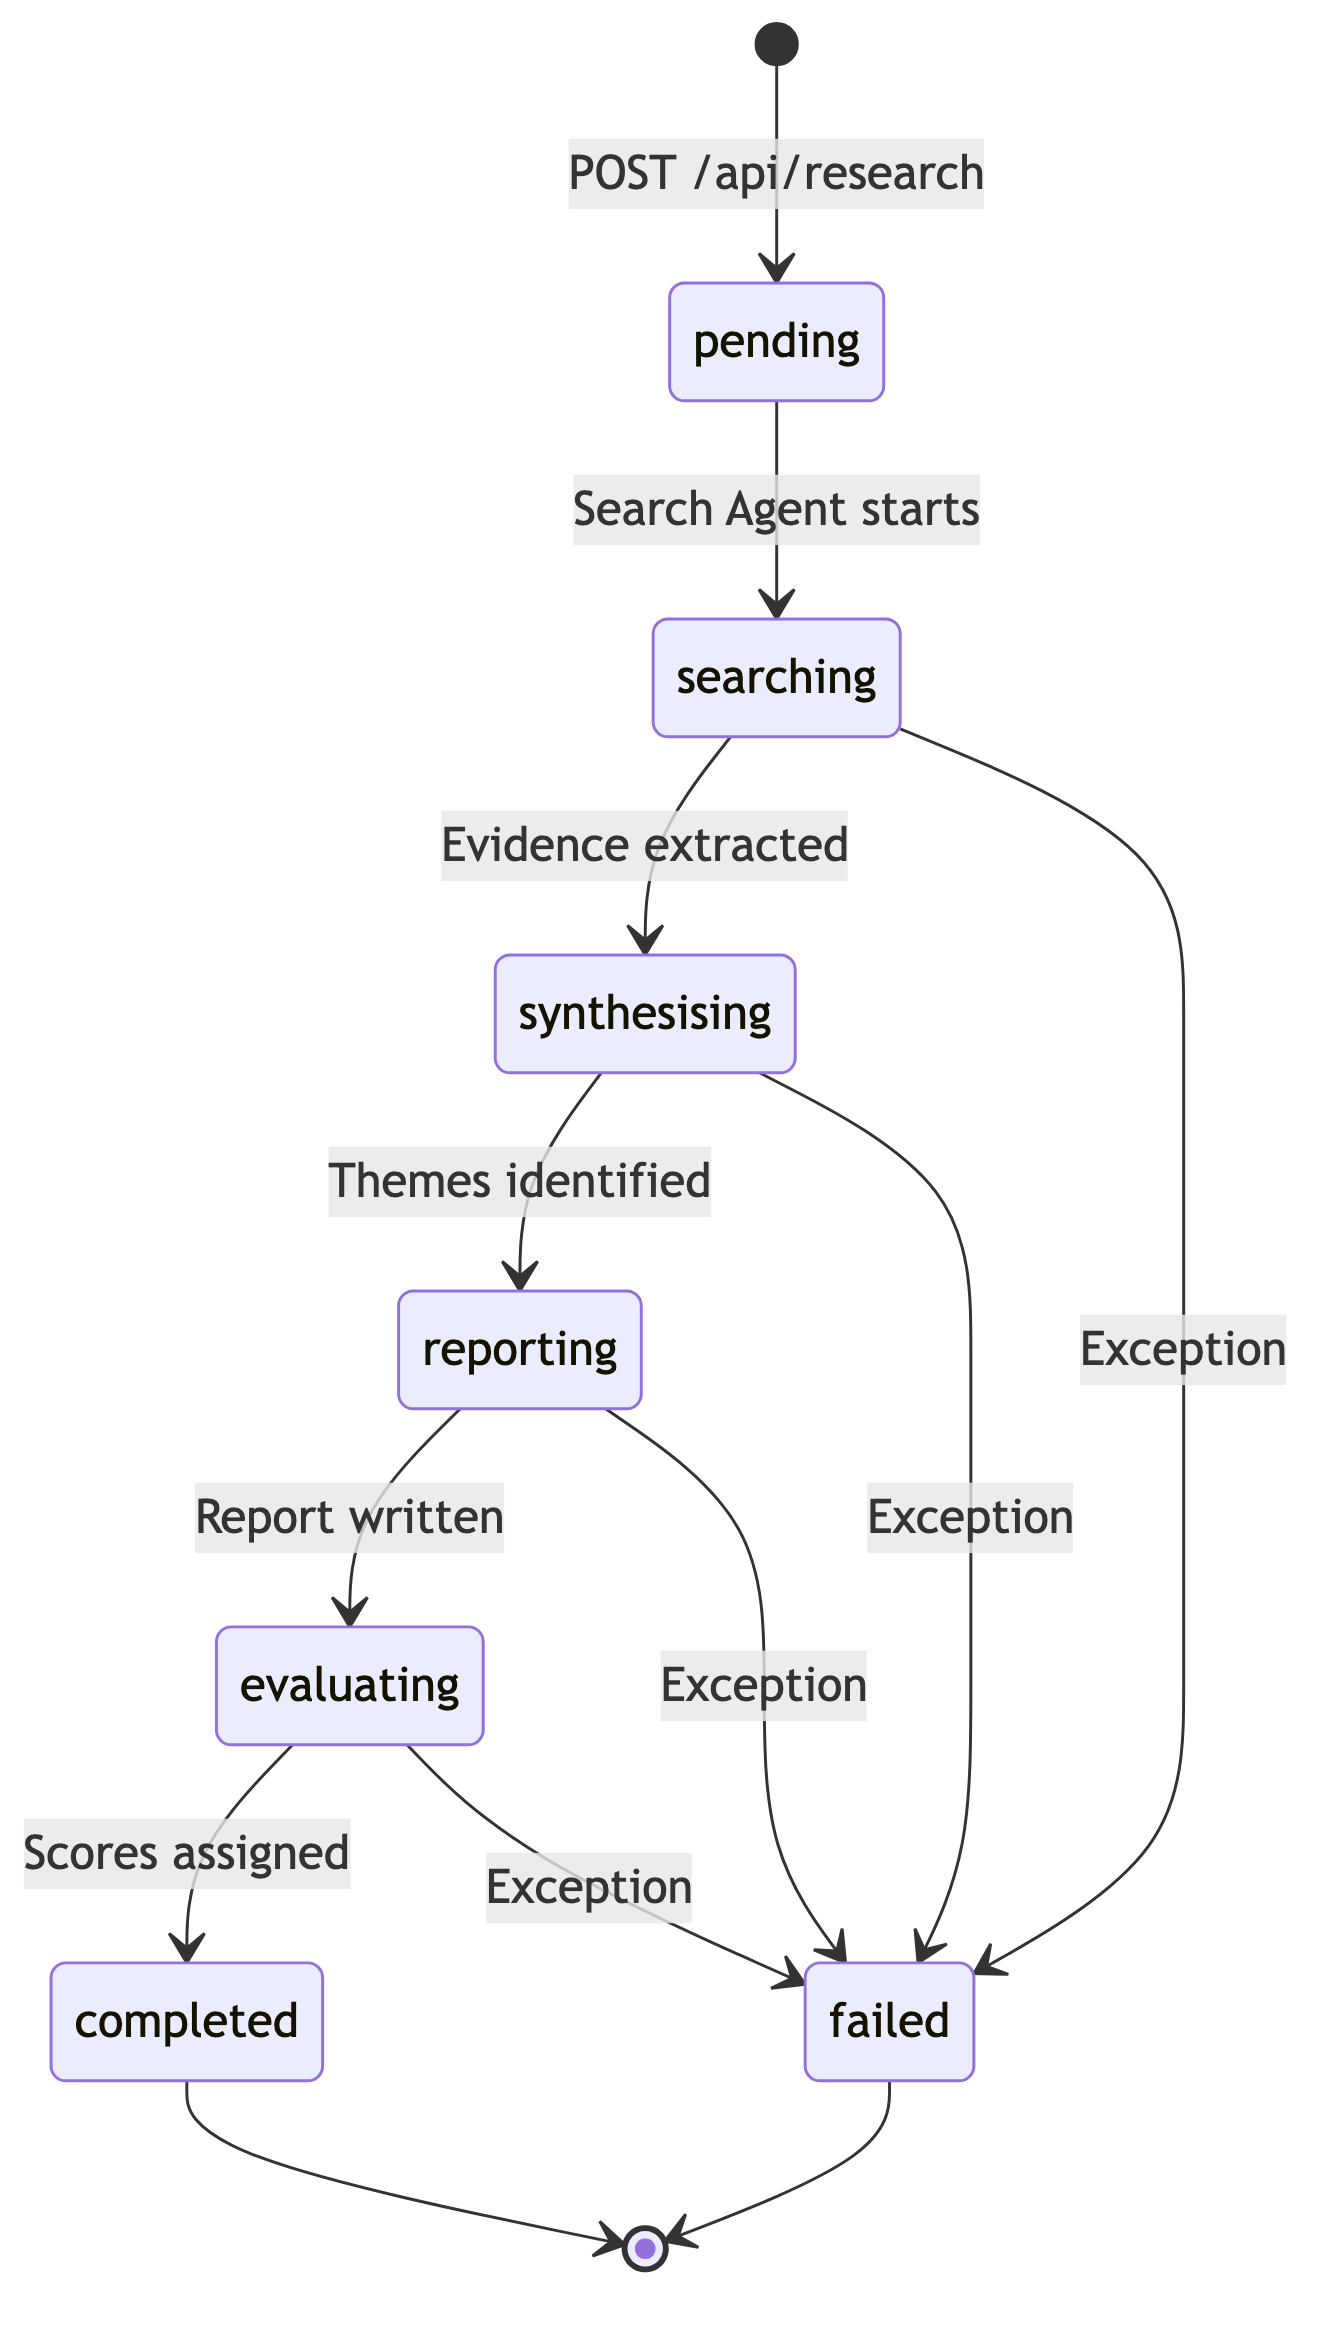
\includegraphics[width=\linewidth]{imgs/report-rendered-8.png}
  \caption{Job status state machine.}
  \label{fig:states}
\end{figure}

\subsection{REST API}

All endpoints except \texttt{/api/health} require \texttt{X-API-Key} when
\texttt{API\_KEY} is set. Key endpoints:

\begin{center}
\small
\begin{tabular}{ll}
  \toprule
  \textbf{Method + Endpoint} & \textbf{Description} \\
  \midrule
  \texttt{POST /api/research}       & Submit question (202) \\
  \texttt{GET  /api/research/\{id\}}  & Status, report, scores \\
  \texttt{GET  .../\{id\}/events}   & SSE live stream \\
  \texttt{GET  .../\{id\}/pdf}      & Download PDF \\
  \texttt{DELETE /api/research}     & Delete all jobs \\
  \texttt{GET  /api/health}         & Health check \\
  \bottomrule
\end{tabular}
\end{center}

% =============================================================================
\section{Frontend}
% =============================================================================

The Next.js~16 frontend (React~19, Tailwind CSS~v4, TypeScript) provides three
pages: \textbf{Home} (submit question, live status, rendered report),
\textbf{History} (all jobs with delete), and \textbf{Job Detail} (full report
with Markdown renderer and PDF download). A \texttt{useJobPoller} hook polls
the REST API every 2\,s and stops on terminal state.

% =============================================================================
\section{Technology Stack}
% =============================================================================

\begin{center}
\small
\begin{tabular}{p{1.7cm} p{2.1cm} p{2.5cm}}
  \toprule
  \textbf{Layer} & \textbf{Technology} & \textbf{Role} \\
  \midrule
  Backend        & Python 3.11+        & Agent \& API logic \\
  API framework  & FastAPI $\geq$0.115 & HTTP, routing, SSE \\
  ASGI server    & Uvicorn $\geq$0.30  & Production server \\
  LLM primary    & Groq SDK            & llama-3.3-70b \\
  LLM fallback   & HuggingFace Hub     & Llama-3.3-70B \\
  Web search     & ddgs / tavily       & DuckDuckGo / premium \\
  Scraping       & httpx + bs4         & Fetch \& parse pages \\
  Validation     & Pydantic $\geq$2    & Typed schemas \\
  Database       & SQLite (WAL)        & Persistent job store \\
  PDF export     & WeasyPrint $\geq$62 & Markdown $\to$ PDF \\
  Frontend       & Next.js 16.2        & React 19 App Router \\
  Styling        & Tailwind CSS v4     & Utility-first CSS \\
  Language (FE)  & TypeScript          & Type safety \\
  Hosting (FE)   & Vercel              & Frontend deployment \\
  \bottomrule
\end{tabular}
\end{center}

% =============================================================================
\section{Design Decisions \& Security}
% =============================================================================

\begin{center}
\small
\begin{tabular}{p{2.0cm} p{4.5cm}}
  \toprule
  \textbf{Decision} & \textbf{Rationale} \\
  \midrule
  Sequential agents   & Each stage depends on the previous stage's typed output. \\
  SQLite + WAL        & Zero operational overhead for single-process demo; clear migration path to PostgreSQL. \\
  \texttt{threading}  & Avoids Redis/Celery dependency; sufficient for sequential jobs. \\
  Temperature 0.3     & Deterministic outputs ease debugging and evaluation. \\
  Dual LLM provider   & Groq (speed) + HuggingFace (fallback) improves availability. \\
  \midrule
  API key auth        & Header \texttt{X-API-Key}; disabled in dev when unset. \\
  CORS allowlist      & Only the configured frontend origin is permitted. \\
  Prompt injection    & No sanitisation layer currently; a production deployment should wrap user input. \\
  \bottomrule
\end{tabular}
\end{center}

% =============================================================================
\section{Deployment}
% =============================================================================

Figure~\ref{fig:deploy} contrasts the current single-instance setup (FastAPI +
SQLite + threads) with a production-scale architecture (load balancer, Celery
workers, PostgreSQL). The frontend is deployed on Vercel; the backend runs via
\texttt{python main.py serve} (Uvicorn). Table~\ref{tab:config} lists the key
environment variables.

\begin{table}[H]
  \centering
  \footnotesize
  \caption{Key environment variables (\texttt{api/.env}).}
  \label{tab:config}
  \begin{tabular}{p{2.9cm} p{0.9cm} p{2.1cm}}
    \toprule
    \textbf{Variable} & \textbf{Default} & \textbf{Purpose} \\
    \midrule
    \texttt{LLM\_PROVIDER}            & auto  & groq / hf / auto \\
    \texttt{GROQ\_API\_KEY}           & —     & Primary Groq key \\
    \texttt{GROQ\_API\_KEY\_2}        & —     & Fallback Groq key \\
    \texttt{HF\_TOKEN}                & —     & HuggingFace token \\
    \texttt{TEMPERATURE}              & 0.3   & LLM temperature \\
    \texttt{TAVILY\_API\_KEY}         & —     & Premium search \\
    \texttt{MAX\_SEARCH\_QUERIES}     & 3     & Queries / question \\
    \texttt{MAX\_RESULTS\_PER\_QUERY} & 5     & Results / query \\
    \texttt{MAX\_CONTENT\_LENGTH}     & 3000  & Chars / page \\
    \texttt{API\_KEY}                 & —     & Auth key \\
    \texttt{CORS\_ORIGINS}            & Vercel URL & Allowed origins \\
    \bottomrule
  \end{tabular}
\end{table}

\begin{figure}[H]
  \centering
  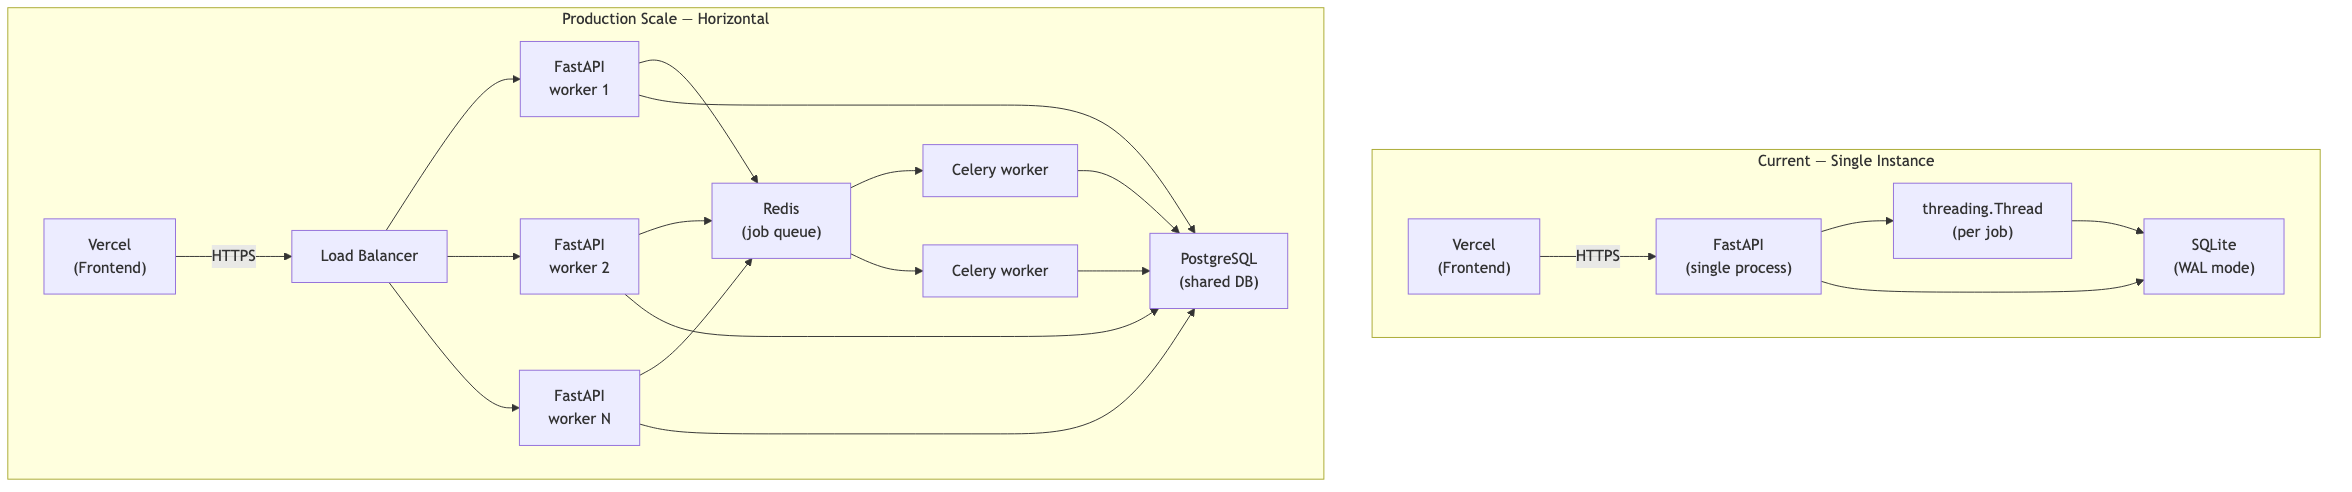
\includegraphics[width=\linewidth]{imgs/report-rendered-12.png}
  \caption{Current vs.\ scalable deployment.}
  \label{fig:deploy}
\end{figure}

% =============================================================================
\section{Limitations \& Future Work}
% =============================================================================

\subsection{Current Limitations}

As a demo prototype, ML-ESS makes several pragmatic trade-offs that constrain
its use beyond supervised settings:

\begin{itemize}
  \item \textbf{No cross-job memory.} Each research job is independent; the
    system cannot reuse evidence gathered in a previous run on a related
    question. A persistent vector store would be needed to enable incremental
    research across sessions.
  \item \textbf{Self-graded evaluation.} The Evaluator uses the same LLM
    that produced the report, introducing circular bias. A separate judge
    model or human annotation loop would improve reliability.
  \item \textbf{Synchronous scraping.} Pages are fetched one at a time
    with \texttt{httpx}; a slow server can add 20–30\,s to the Search Agent
    phase. An async fetch with \texttt{asyncio.gather} would cut this by
    $3\times$.
  \item \textbf{No source credibility verification.} Credibility notes are
    LLM-generated heuristics — not checked against domain authority, publication
    date, or peer-review status.
  \item \textbf{SQLite concurrency ceiling.} WAL mode allows multiple
    concurrent readers but only one writer. Under sustained load (many
    simultaneous jobs), write operations queue up.
  \item \textbf{No prompt injection protection.} User questions are passed
    verbatim to LLM prompts. A production deployment should wrap input in a
    trusted envelope.
\end{itemize}

\subsection{Planned Extensions}

\begin{itemize}
  \item Streaming LLM output (token-by-token SSE) to reduce perceived latency.
  \item Async parallel scraping with \texttt{asyncio.gather}.
  \item Cross-job knowledge base via ChromaDB or pgvector.
  \item Independent evaluator model for unbiased quality scoring.
  \item Human-in-the-loop evidence annotation before report generation.
  \item Multi-language output via a dedicated translation agent.
  \item Horizontal scaling path: Redis job queue, Celery workers, PostgreSQL.
\end{itemize}

% =============================================================================
\section{Conclusion}
% =============================================================================

ML-ESS demonstrates that a small, well-structured multi-agent system can
automate the full research pipeline — from a natural language question to a
cited, evaluated report — in minutes. As a demo prototype it prioritises
transparency over scale: all intermediate artefacts are persisted and
inspectable, and the pipeline can be traced end-to-end without hidden state.
Its modular design is its central principle: \emph{a correct, auditable core
that grows incrementally}. Inserting a new agent requires adding one function
and extending \texttt{SharedState}; the REST API and frontend adapt
automatically.

\section*{Acknowledgements}
The authors thank the AIMS Research Innovation Centre and the organisers of the
2026 Doctoral Training School for the research environment and computational
resources.

% =============================================================================
\begin{thebibliography}{9}

\bibitem{rag}
P. Lewis \textit{et al.}, ``Retrieval-Augmented Generation for
Knowledge-Intensive NLP Tasks,'' \textit{NeurIPS}, vol.~33, 2020,
pp.~9459--9474.

\bibitem{autogpt}
T. Significant Gravitas, \textit{AutoGPT}, GitHub, 2023.
\url{https://github.com/Significant-Gravitas/AutoGPT}

\bibitem{crewai}
J. Moura, \textit{CrewAI}, GitHub, 2024.
\url{https://github.com/joaomdmoura/crewAI}

\bibitem{langchain}
H. Chase, \textit{LangChain}, GitHub, 2022.
\url{https://github.com/langchain-ai/langchain}

\bibitem{llama3}
Meta AI, ``The Llama 3 Herd of Models,'' \textit{arXiv:2407.21783}, 2024.

\bibitem{fastapi}
S. Ramirez, \textit{FastAPI}, 2019. \url{https://fastapi.tiangolo.com}

\end{thebibliography}

\end{document}
